\chapter{下置硅光栅反射镜的氮化硅光栅耦合器}\label{chap:3}


\section{光栅耦合器的理论基础}


\begin{figure}[!htbp]
    \centering
    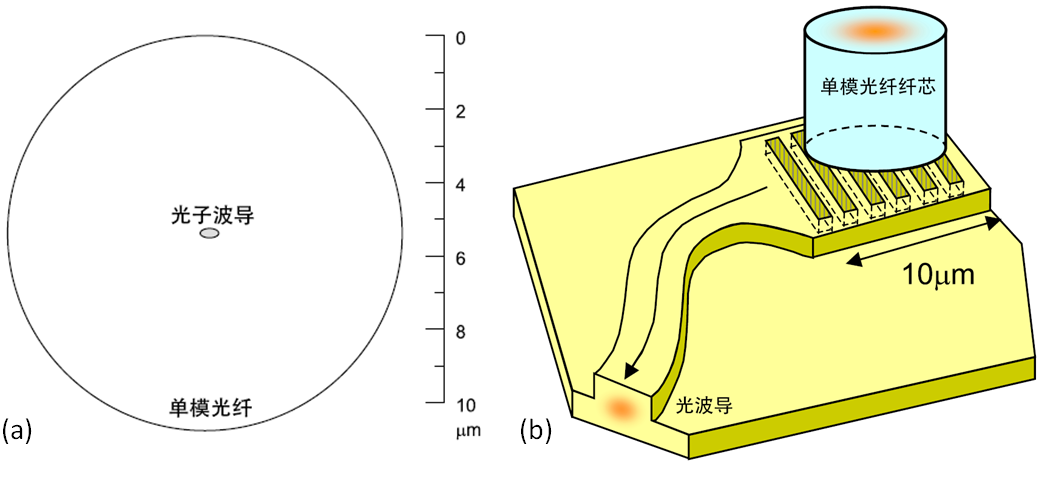
\includegraphics[width=1\textwidth]{Img/3-1.png}
    \caption{单模光纤的纤芯尺寸与光子波导的尺寸相差一个数量级,光从单模光纤很难直接耦合到光波导中,常用透镜光纤、倒锥模斑转换器或光栅耦合器来辅助耦合。(b)常见的光栅耦合器的结构示意图,通过光栅的衍射,改变光的传播方向,实现单模光纤与光波导之间的光耦合。\cite{Dirkgrating}}
    \label{fig:3-1}
\end{figure}
%%%%%%%%%%%%%%%%%%%%%%%%%%%%%%%%%%%%%%%%%%%%%%%%%%%%%%%%%%%%%%%%%%%%%%%%%%%%%%%%%%%%%%%%%%%%%%%%%%%%%%%%%%%%%%%%%%%%%%

在光子集成芯片中,片上的集成光学元器件通过微米量级的线波导进行光的连接。根据国际电信联盟ITU制定的标准单模光纤标准(G.652)\cite{smf},标准单模光纤的模场直径(mode field diameter)为10.4$\mu$m,相比微米量级的光波导相比,光纤纤芯尺寸和光波导尺寸相差一个数量级,如图3.1a所示。

因此,光从单模光纤到光波导之间的光耦合,不能直接相接,需要借助特殊设计的光耦合器实现光能量和信息的传输。常见的光耦合器有透镜光纤(Lensed-fiber)、缓变倒锥的模斑转换器(Spot-size convertor)\cite{Shoji2002Low,Sharee2003Ultra}和光栅耦合器(Grating coupler)等。

光栅耦合器的整体尺寸与单模光纤的纤芯直径接近($\sim$10$\mu$m),如图3.1b所示。光从单模光纤垂直输入到光子集成芯片的表面,受到光栅的衍射作用,改变传播方向,耦合到光波导中。

一方面,解决了光从单模光纤到光波导模场直径的巨大差异,实现了高效率的耦合;另一方面,光栅耦合器是一种非接触式的垂直光耦合,相比透镜光纤和模斑转换器,可以在无需晶元解理的情况下,实现光子芯片的片上测试,具有更加便利的测试场景,这也是光栅耦合器垂直耦合相比端面耦合的一个优势。\cite{Dirkgrating}

\begin{figure}[!htbp]
    \centering
    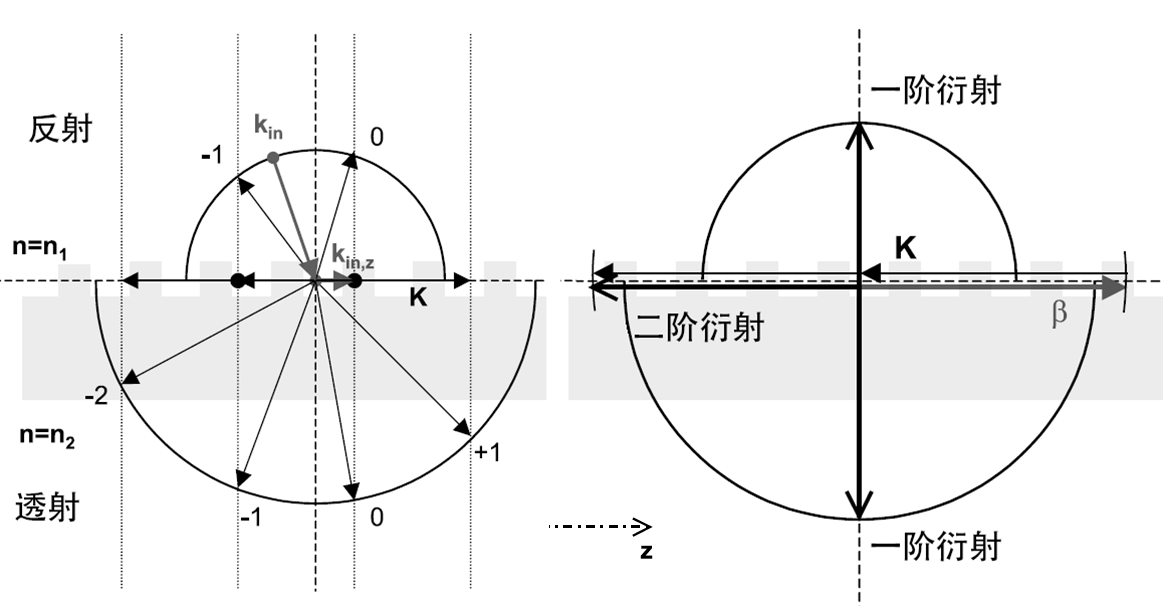
\includegraphics[width=1\textwidth]{Img/3-2.png}
    \caption{(a)一般的光栅界面衍射,光栅的上下两端具有不同折射率,倾斜角度入射的光发生光栅衍射时光波矢满足的布拉格条件。(b)一般光栅界面衍射的特殊情况,当入射的光平行于光栅表面时的衍射情况。当光栅调制的波矢等于入射的光波导模式的有效传播常数β时,可实现垂直光栅表面的一阶衍射。\cite{Dirkgrating}}
    \label{fig:3-2}
\end{figure}
%%%%%%%%%%%%%%%%%%%%%%%%%%%%%%%%%%%%%%%%%%%%%%%%%%%%%%%%%%%%%%%%%%%%%%%%%%%%%%%%%%%%%%%%%%%%%%%%%%%%%%%%%%%%%%%%%%%%%%

在体光学的范畴中,光栅是一种常见的大量等宽等间距的平行狭缝构成的,可以在波矢空间对光进行调制的一种衍射光学元件。

如图3.2a,为一般化的光栅界面衍射情况,在光栅界面的上下两端具有$n_1$和$n_2$两种不同折射率的材料,则对于真空中波矢为$k_0$的入射光,其在界面的透射和反射光的波矢z分量(z方向为沿着光栅的方向)满足如下的布拉格方程:
\begin{equation}
k_{transmission,z}= k_{incidence,z}  + mK
\end{equation}
\begin{equation}
k_{reflection,z}= k_{incidence,z}  + mK
\end{equation}
其中kz为入射、反射或透射光的波矢的z分量,而$|K| = 2\pi/\Lambda $,是衍射光栅的波矢,m为光栅的衍射级数。
\begin{equation}
k_{reflection}=k_{incidence}=k_0⋅n_1
\end{equation}
\begin{equation}
k_{transmission}=k_0⋅n_2
\end{equation}
因此反射和透射的衍射光的波矢落在以$k_0n_1$和$k_0n_2$为半径的两个半圆中。

其中,0级衍射级没有受到光栅的波矢调制作用,满足传统的Sneal定律。而-2,-1,1,2级衍射级代表受到光栅衍射后的各个衍射级。如图3.2a所示,通过布拉格条件可以简单的计算出光经过光栅衍射后,在各个衍射级上的反射和透射的方向。

当然,也有特殊情况,如图3.2b,当入射光的波矢平行于光栅界面时,如光在集成光子芯片表面的光波导上传输,则此时入射光的波矢kz等于光在波导中的模式传播常数$\beta$,即
\begin{equation}
k_{transmission,z}= \beta + mK
\end{equation}
\begin{equation}
k_{reflection,z}= \beta + mK
\end{equation}
则如图3.2b,当光栅的波矢 $|K| =\beta$时,可以实现垂直的一阶衍射,满足垂直耦合的需求。此外,存在一个与入射波矢相反方向的二阶衍射,因此,通常的光栅耦合器,通常避免垂直90°的耦合角度,以避免二阶衍射带来的反射,通常采用略微倾斜的耦合角度(如图3.3,通常为5$\sim$20°不等)。此外,倾斜的耦合角度也有利于芯片测试时光纤夹具的摆放。

对于光栅耦合器,有几个常用的性能指标,用于表征器件的性能:\cite{Dirkgrating,Kevingrating}

①、耦合效率或插入损耗:光波导传输模式的光功率为$P_1$,而耦合到单模光纤模式时光功率为$P_2$。或者反过来,单模光纤传输模式的光功率为$P_1$,而耦合到光波导模式时光功率为$P_2$,则其耦合效率百分率$\eta$:
\begin{equation}
\eta = \frac{P_2}{P_1} \times 100\% 
\end{equation}
转为对数形式,其插入损耗IL为
\begin{equation}
IL = 10\times log_{10}{\frac{P_2}{P_1}}  [dB]
\end{equation}

②、1dB或3dB带宽:对于光栅耦合器,其设计的中心波长的一般具有最高的耦合效率或最低的插入损耗。而当波长偏移了中心波长时,插入损耗将随之增加。当插入损耗增加了1dB或3dB时,其对应的波长偏移的上限和下限形成的波长范围,即为光栅耦合器的1dB或3dB带宽。光栅耦合器的1dB带宽往往要求≥50nm,以满足红外光通信C波段或L波段的全波段覆盖。

③、模式或偏振相关损耗:波导中存在较为常用的几组偏振状态不通的模式,如TE模式或TM模式。光栅耦合器的设计往往只针对单一模式或少数的模式。不同偏振或模式之间的耦合效率的偏差,即为模式或偏振相关损耗。通常情况下,有专门设计的光栅耦合器,以提升多个模式或偏振的耦合效率,以降低模式或偏振相关损耗,来实现模式复用下的高效率耦合。也有专门设计的光栅耦合器,来提升模式或偏振相关损耗,只耦合需要的模式,抑制非需要的模式。本论文中只考虑最低阶的TE0基础模式,暂不考虑TM模式。


\begin{figure}[!htbp]
    \centering
    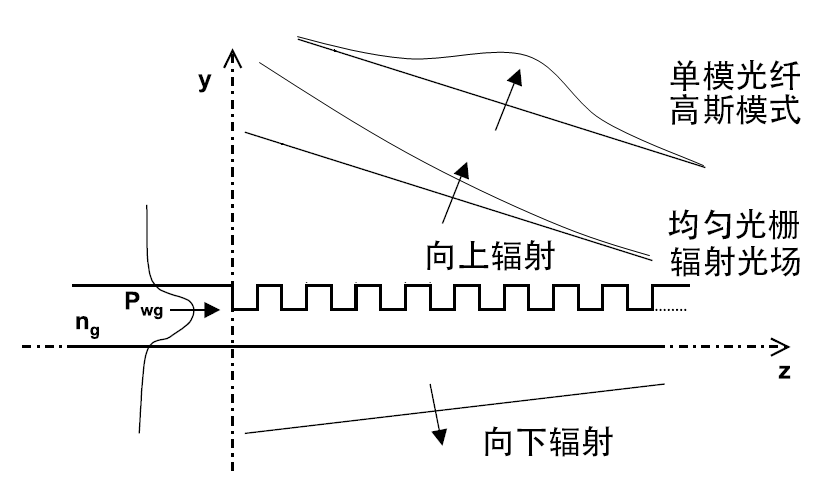
\includegraphics[width=1\textwidth]{Img/3-3.png}
    \caption{光栅耦合器的高性能的关键。光从波导中传输到光栅处,受光栅衍射作用向上辐射和向下辐射。均匀光栅的辐射光场近似为能量指数衰减的光场,其中只有匹配单模光纤高斯模式的部分可以实现耦合。}
    \label{fig:3-3}
\end{figure}
%%%%%%%%%%%%%%%%%%%%%%%%%%%%%%%%%%%%%%%%%%%%%%%%%%%%%%%%%%%%%%%%%%%%%%%%%%%%%%%%%%%%%%%%%%%%%%%%%%%%%%%%%%%%%%%%%%%%%%

图3.3为传统设计的光栅耦合器,在光波导上刻蚀光栅,实现光的1阶衍射。由于光栅的1级衍射级在材料界面的两端都存在,因此,光栅的衍射不仅向上辐射,同时也向下辐射,两端的同时辐射意味着将损失接近一半的光功率,不利于耦合效率的提升。

因此,对于高性能光栅耦合,往往需要特殊设计的光栅耦合器的方案,来提高光的方向性,一方面要避免光栅的向下衍射的辐射损耗,换言之,需要提高光栅的向上辐射的方向选择性,进而提升光栅耦合器的耦合效率。

另一方面,对于均匀光栅而言,随着光栅向上辐射能量,光在波导中的功率逐渐减少。因此向上辐射的光场一般呈现指数衰减的趋势,如图3.3所示,均匀光栅的指数衰减辐射光场,与标准单模光纤的类高斯模式的光场,存在模式失配,只有模式匹配的部分功率可以耦合到单模光纤中,因此,效率受到限制。需要适当修整向上辐射的光场分布,采用特殊设计的非均匀的非均匀光栅,匹配单模光纤的高斯模式,提高耦合效率。

近年来,随着氮化硅材料的气相外延生长和等离子体加工工艺的逐渐成熟,基于氮化硅的光子集成芯片和器件逐渐成为研究的热门。氮化硅作为一种新兴发展的光子集成材料体系,相比传统硅的光子集成材料而言,具有低损耗、较低的折射率、高加工容差、低热光系数,低双光子吸收、可见光波段透明等优异的材料特性,具有优异的应用潜力,可用于制备低损耗、低串扰、高加工容差等的更具应用竞争力的光子集成芯片。\cite{Yang2016Ultra,Subramanian2016Silicon,Rahim2017Expanding,Mu2017Silicon}

然而,氮化硅的光子集成材料体系中,很难制备高性能的氮化硅光栅耦合器。一方面,由于氮化硅的折射率比较低(n$\sim$2),往往需要深刻蚀的氮化硅光栅才能实现较高的光栅辐射强度;另一方面,深刻蚀的氮化硅光栅的向上辐射选择性较差,有接近一半的光功率会被损失,因此很难实现较高的耦合效率。

相比硅材料,由于硅材料先天具有高折射率的优势(n$\sim$3.42),在刻蚀的硅光栅耦合器中,硅与氧化硅包层可以形成较高的折射率反差,使得硅光栅齿具有较高的辐射强度,通过浅刻蚀的硅光栅便可以实现较高的向上辐射效率,具有更高的耦合效率。此外,还可以通过非均匀光栅的方式,在单模光纤纤芯直径的范围($\sim$10.4$\mu$m)实现辐射光场的模式匹配,进一步的提升耦合效率。

综上所述,较低折射率的氮化硅介质材料,要想实现类似于硅基光栅耦合器的高耦合效率,一方面需要提升向上辐射的功率,即打破竖直方向的辐射对称性;另一方面是提高光栅辐射光场到单模光纤的耦合效率,即模式匹配。

\section{高性能光栅耦合器的调研}


\begin{table}[!htbp]
    \caption{已发表的高性能氮化硅光栅耦合器的设计方案、性能和加工复杂度对比。}
    \label{tab:1}
    \centering
    \footnotesize% fontsize
    \setlength{\tabcolsep}{4pt}% column separation
    \renewcommand{\arraystretch}{1.2}%row space 
\begin{tabular}{ccccccc}
设计方案          &1dB带宽 & 峰值功率  & 刻蚀步骤 & CMP & 精准套刻 & 文献       \\ \hline
传统光栅          & 50    & -5.8   & 1    & ×   & ×    & \cite{Shainline2017Room}     \\
传统光栅          & 60    & -5.1   & 1    & ×   & ×    & \cite{Zhang2014High} \\
传统光栅          & 67    & -4.2   & 1    & ×   & ×    & \cite{Doerr2010Wide} \\
波导倒锥          & 54    & -3.7   & 2    & ×   & √    & \cite{Cheng2016Compact} \\
下置DBR反射镜      & 53    & -2.5   & 1    & ×   & ×    & \cite{Huijuan2014Efficient} \\
下置硅光栅反射镜      & 80    & -1.3   & 3    & √   & √    & \cite{Sacher2014Wide}\\
下置硅光栅反射镜      & 40    & -0.88* & 2    & √   & √    & \cite{Jinghui2015Ultra} \\
阶梯状光栅齿        & 20    & -1.5   & 2    & ×   & √    & \cite{Chen2016High,Chen2017Experimental} \\
下置硅光栅反射镜     & 65    & -2.5   & 1    & ×   & ×    & 本论文      \\
\multicolumn{7}{c}{*号标记代表结果是仿真结果}        
\end{tabular}
\end{table}
%%%%%%%%%%%%%%%%%%%%%%%%%%%%%%%%%%%%%%%%%%%%%%%%%%%%%%%%%%%%%%%%%%%%%%%%%%%%%%%%%%%%%%%%%%%%%%%%%%%%%%%%%%%%%%%%%%%%%%
%%%%%%%%%%%%%%%%%%%%%%%%%%%%%%%%%%%%%%%%%%%%%%%%%%%%%%%%%%%%%%%%%%%%%%%%%%%%%%%%%%%%%%%%%%%%%%%%%%%%%%%%%%%%%%%%%%%%%%
%%%%%%%%%%%%%%%%%%%%%%%%%%%%%%%%%%%%%%%%%%%%%%%%%%%%%%%%%%%%%%%%%%%%%%%%%%%%%%%%%%%%%%%%%%%%%%%%%%%%%%%%%%%%%%%%%%%%%%

传统的氮化硅光栅耦合器,指只在氮化硅波导上刻蚀光栅结构的光栅耦合器,器件简单,便捷,易加工,在实际的光子集成芯片系统中较为常见。如上节所述,由于氮化硅较低的折射率的限制,传统的氮化硅光栅耦合器很难同时满足“较高的向上辐射方向选择性”和“与单模光纤高斯模式的高度匹配”的高效率耦合的需求。

因此,如表3-1所示,由美国国家标准与技术研究院NIST的Jeffrey M. Shainline等人和美国贝尔实验室Bell等的Christopher R. Doerr等人报道的传统的氮化硅光栅耦合器,虽然具有较宽的1dB带宽(>60nm),然而其普遍的光耦合效率低于 -4 $\sim$ -5dB \cite{Shainline2017Room,Zhang2014High,Doerr2010Wide}。对于无源集成光子芯片而言,光从单模光纤耦合到芯片再耦合回单模光纤,即单模光纤→光子芯片→单模光纤,两次耦合则总的耦合损耗将达到-8 $\sim$ -10dB,即便氮化硅的光子芯片具有较低的片上传输损耗,在通信应用中,较大的耦合损耗对信噪比和通信质量存在较为严重的影响。

为提升氮化硅光栅耦合器的耦合效率,通过查阅高性能氮化硅光栅耦合器的文献,分析已发表的高性能氮化硅光栅耦合器的提升效率的方案,如图3.4所示,列举了几个有影响力的氮化硅高效率光栅耦合器。其对应的氮化硅光栅耦合器的性能指标、设计方案、峰值功率、加工复杂度等信息列举在表3-1中,加工复杂度转有光栅的刻蚀步骤次数、是否需要化学机械抛光CMP,是否需要高精度的电子束套刻曝光等信息。

在表3-1中,已知的有效提升氮化硅光栅耦合器的设计方案,大致可以归结为下置分布式布拉格光栅DBR反射镜方案、下置金属反射镜、下置的光栅反射镜方案、上置高折射率光栅覆盖层和特殊向上辐射光栅结构等方案。对应的高性能光栅耦合器设计方案的简图如图3.5所示。

通过调研已发表的器件方案的优缺点,从中寻找合适的器件设计灵感。

\begin{figure}[!htbp]
    \centering
    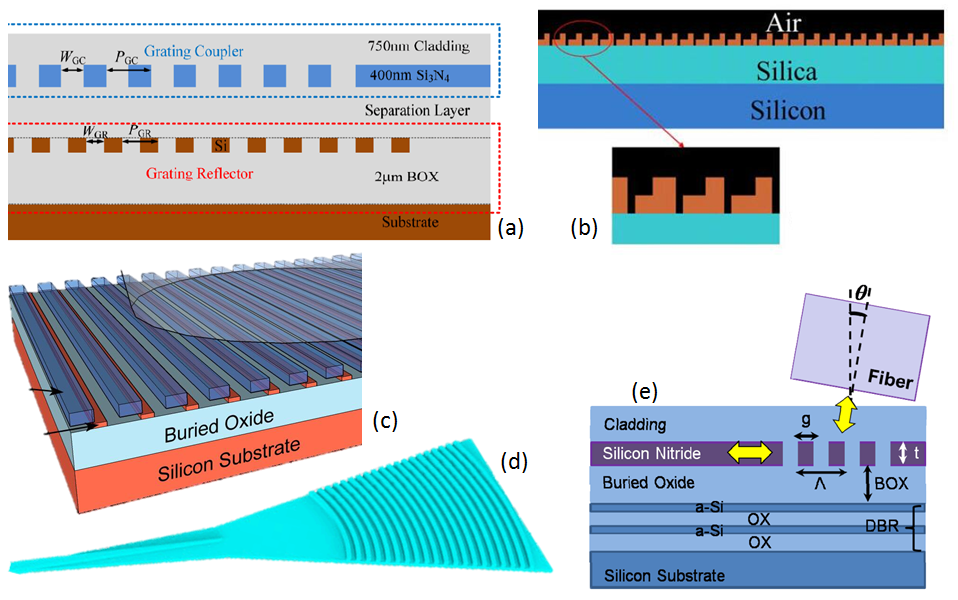
\includegraphics[width=1\textwidth]{Img/3-4.png}
    \caption{ SiNx光栅耦合器的文献调研(a)华中科技大学的硅光栅反射镜+氮化硅光栅耦合器方案。(b) 浙江大学的阶梯状光栅和远距离辐射角度映射方案。 (c) 多伦多大学的硅光栅反射镜+氮化硅光栅耦合器方案。(d)华中科技大学的倒锥浅刻蚀方案。 (e) 新加坡A*STAR的下置DBR反射镜方案。\cite{Cheng2016Compact,Huijuan2014Efficient,Sacher2014Wide,Jinghui2015Ultra,Chen2016High}}
    \label{fig:3-4}
\end{figure}
%%%%%%%%%%%%%%%%%%%%%%%%%%%%%%%%%%%%%%%%%%%%%%%%%%%%%%%%%%%%%%%%%%%%%%%%%%%%%%%%%%%%%%%%%%%%%%%%%%%%%%%%%%%%%%%%%%%%%

\begin{figure}[!htbp]
    \centering
    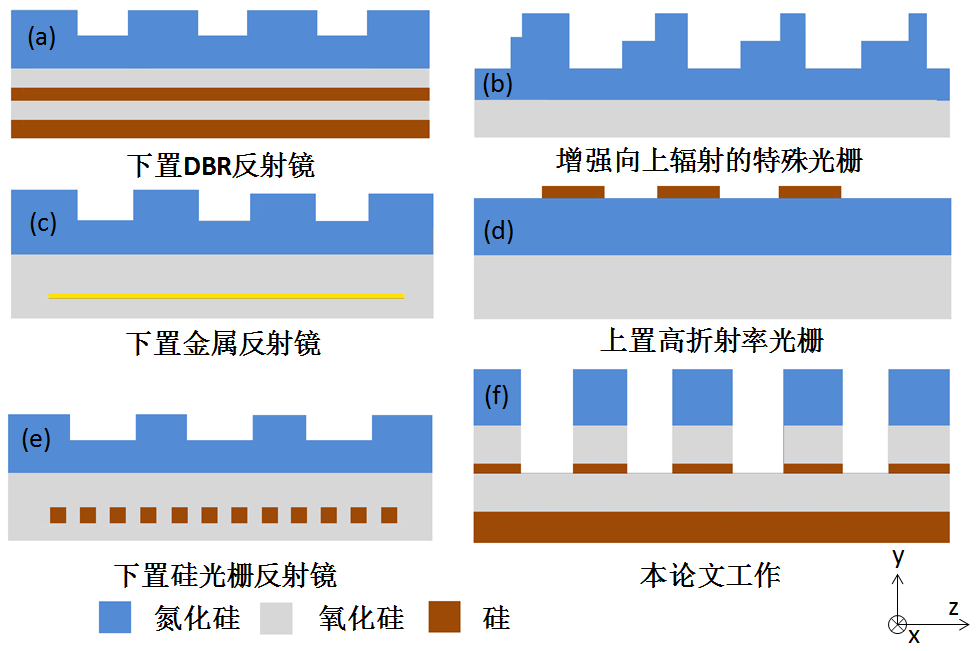
\includegraphics[width=1\textwidth]{Img/3-5.png}
    \caption{已发表的高性能氮化硅光栅耦合器的设计方案简图。(a)通过交替生长高折射率和低折射率材料的下置DBR反射镜方案、(b)通过多次对准刻蚀形成的增强向上辐射的特殊光栅方案、(c)通过沉积高反射率金属形成的下置金属反射镜方案、(d)通过沉积高折射率光栅覆盖层代替氮化硅光栅的方案、(e)通过下置的高反射率亚波长硅光栅的方案。}
    \label{fig:3-5}
\end{figure}
%%%%%%%%%%%%%%%%%%%%%%%%%%%%%%%%%%%%%%%%%%%%%%%%%%%%%%%%%%%%%%%%%%%%%%%%%%%%%%%%%%%%%%%%%%%%%%%%%%%%%%%%%%%%%%%%%%%%%%

下置DBR的方案,需要在氮化硅光栅的下端交替沉积四分之一波长厚度的高折射率和低折射率的介质材料,其中,高折射率材料通常是非晶硅、低折射率材料通常是氧化硅。需要足够多的DBR周期数来形成有效的反射,如新加坡A*STAR的Huijuan Zhang等人采用了两个周期的DBR形成较高底部反射率,实现了-2.5dB的插入损耗。DBR反射镜是通过布拉格条件形成反射,其布拉格反射条件对波长有较强的选择性,因此光栅耦合的1dB带宽相比传统的氮化硅光栅耦合器较窄一些。

增强向上辐射的特殊光栅,通过特殊的光栅齿结构,如图3.4b和3.5b所示的台阶状光栅等,使得辐射的光倾向于向上辐射,也可以极大的提升向上辐射的功率。浙江大学Yang Chen等人的通过阶梯状光栅和远距离辐射角度映射的方法,实现-1.5dB的耦合效率和60nm的3dB带宽\cite{Chen2016High,Chen2017Experimental}。耦合效率很高,而器件带宽稍低,而且器件的测试中,需要将光纤放置在较高位置,与传统的光栅耦合器的测试和封装方式不太兼容。此外,特殊的阶梯状光栅需要极其严格的版图对准套刻过程,对器件的加工提出了更严格的要求,对良品率造成挑战。

通过下置的金属反射镜,如图3.5c中所示,器件结构相对简单,金属具有宽光谱的光反射特性,通过金属层的反射,也能实现高性能的光栅耦合器。金属层的反射与光波长无关,因此器件1dB带宽也较宽。然而需要预先在氮化硅波导的下端沉积一层金属反射层。预先沉积金属的步骤,与传统的CMOS工艺的金属化流程不一致,金属的沉积也会为后续的电子束器件曝光等工序增加不可控的因素等,邻近效应修正会发生变化。

上置的高折射率光栅的方案也可以很好的实现提升耦合效率的方式,如图3.5d,可以在无需刻蚀氮化硅波导的情况下,通过高折射率光栅代替氮化硅光栅实现耦合。采用了类似的方法设计了铌酸锂的光栅耦合器,铌酸锂的折射率与氮化硅类似,通过上置的高折射率非晶硅光栅,在无须刻蚀铌酸锂波导的情况下,实现$-$3.06dB高效率和55nm的1dB带宽的光耦合效率,详情参见简健的博士论文。

除上述的光栅耦合器方案外,具有高的耦合效率和宽的1dB带宽,方法简便可靠的是由华中科大的Jinghui Zou和多伦多大学的Wesley D. Sacher等人报道的下置硅光栅反射镜的方案,如图3.4a,3.4c和3.5e所示\cite{Sacher2014Wide,Jinghui2015Ultra}。下置硅光栅反射镜,通过在传统的氮化硅光栅耦合器的光栅下端,引入亚波长的高折射率的硅光栅,通过硅光栅形成极高的发射率,提高氮化硅光栅耦合器的耦合效率。相比下置多层DBR反射器的光栅耦合器方案,一方面,硅光栅反射镜具有更高的反射率,可以实现更高的效率;另一方面,亚波长的硅光栅反射镜相比DBR而言,波长选择性较小,可以实现更宽的1dB带宽。此外,下置的硅光栅反射镜可以采用商用的绝缘层上硅SOI晶片的高质量的单晶硅来制备,避免DBR需要通过多次的非晶硅的气相沉积,有利于制备的器件的性能稳定,可靠,高效。如表3-1所示,下置硅光栅反射镜的方案可以达到理论的 -1.3dB和-0.88dB的极低插入损耗,1dB带宽也达到相应的80nm和40nm。

\begin{figure}[!htbp]
    \centering
    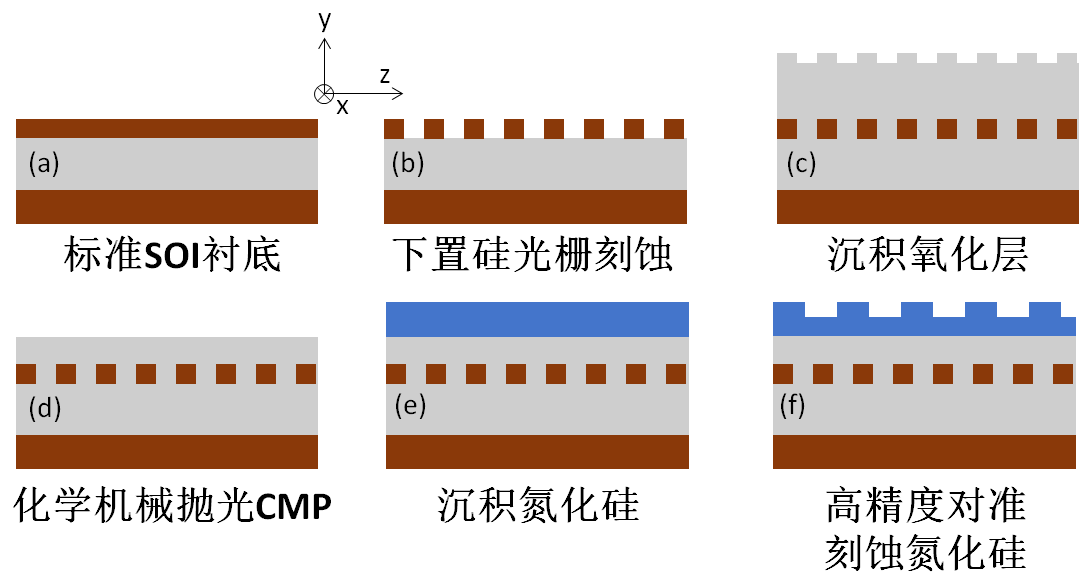
\includegraphics[width=1\textwidth]{Img/3-6.png}
    \caption{下置硅光栅反射镜的光栅耦合器的复杂加工流程。(a)选用商用的SOI晶片。(b)通过电子束光刻EBL和等离子体刻蚀制备硅光栅反射镜。(c)沉积二氧化硅氧化层。(d) 化学机械抛光CMP,形成平整的表面。(e)沉积氮化硅。(f) 通过高精度的对准曝光,刻蚀制备氮化硅光栅。}
    \label{fig:3-6}
\end{figure}
%%%%%%%%%%%%%%%%%%%%%%%%%%%%%%%%%%%%%%%%%%%%%%%%%%%%%%%%%%%%%%%%%%%%%%%%%%%%%%%%%%%%%%%%%%%%%%%%%%%%%%%%%%%%%%%%%%%%%%

下置硅光栅反射镜方案具有显著突出的效果,然而,下置硅光栅的耦合器方案的器件制备过程比较复杂,如图3.6所示。制备过程中,不仅需要使用化学机械抛光CMP进行表面平整化,还需要高精准度的EBL对准曝光,过程繁杂,对加工精度要求高,误差容忍度较差。在实际的复杂光子芯片制备中,复杂低误差容忍度的加工流程会导致成品率降低,缺乏足够的可行性。\cite{Hochberg2010Towards}

\section{基于一次刻蚀的高性能光栅耦合器}

\subsection{器件设计方案}

\begin{figure}[!htbp]
    \centering
    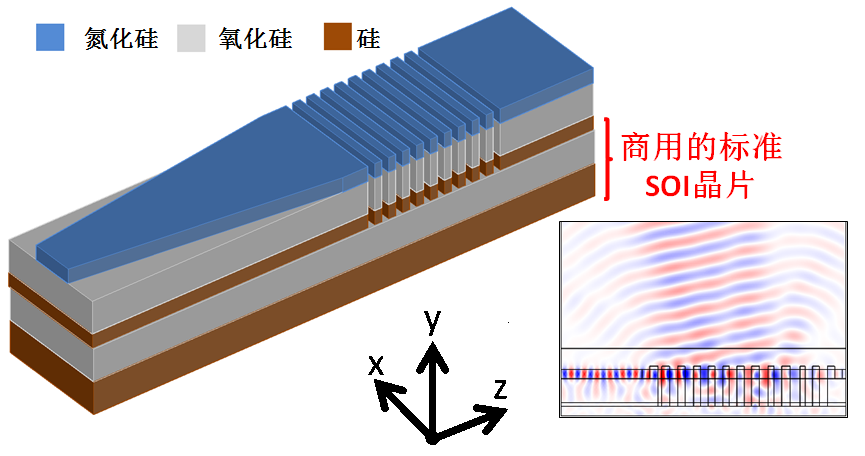
\includegraphics[width=1\textwidth]{Img/3-7.png}
    \caption{一步刻蚀的下置硅光栅反射镜的氮化硅光栅耦合器。电场插图展示了从波导左端输入光模式的情况下,可以实现较好的向上辐射并匹配单模光纤的模式。}
    \label{fig:3-7}
\end{figure}
%%%%%%%%%%%%%%%%%%%%%%%%%%%%%%%%%%%%%%%%%%%%%%%%%%%%%%%%%%%%%%%%%%%%%%%%%%%%%%%%%%%%%%%%%%%%%%%%%%%%%%%%%%%%%%%%%%%%%%
如上一节所述,受下置硅光栅反射镜的光栅耦合器方案启发,为了避免CMP化学机械抛光和高精度EBL对准曝光等繁杂的器件加工流程,在兼顾下置硅光栅反射镜方案的高性能前提下,提出了一种通过单次等离子体刻蚀,实现氮化硅和硅的光栅同步制备的光栅耦合器方案,既有效提升耦合效率,又避免了器件的复杂制备流程。

如图3.7所示,提出的单次刻蚀的下置硅光栅反射的氮化硅光栅耦合器的器件结构相对简单,器件的制备基于商用的SOI晶片。在SOI晶片的上方沉积二氧化硅和氮化硅波导层后,通过一步刻蚀的方式,刻穿氮化硅、二氧化硅和硅层,同时形成上部的氮化硅光栅以及下置的硅光栅反射镜,无须CMP和高精度的对准套刻。

上层的氮化硅衍射光栅用于辐射氮化硅波导中传输的光模式,而下置的硅光栅反射层,用于反射向下辐射的光功率部分,使得波导中的光整体向上辐射,避免了向下辐射带来的耦合效率损失。

图3.7的插入图为光栅耦合器仿真的电场辐射图,通过仿真证实了在一步刻蚀的氮化硅光栅耦合器和硅光栅反射镜的双重作用下,可以使氮化硅波导中传输的TE模式光,直接向上辐射,并较好地匹配单模光纤的模式,实现高的耦合效率和宽的1dB带宽。

综上所述,提出的方案具有简单便捷,无需CMP抛光和EBL高精度对准曝光、以及宽带高效率的特点,简单便捷的器件加工步骤在复杂的光子芯片制作中具有更加广阔的应用前景。

\subsection{器件仿真}

在选定了一步刻蚀的光栅耦合器方案后,需要通过仿真进行具体的器件参数设计和优化,通过仿真可靠性、遗传算法引入和后期数据处理的需要,采用有限元的电磁场频域求解器对器件进行设计和优化。\cite{Bathe2000Finite}

\begin{figure}[!htbp]
    \centering
    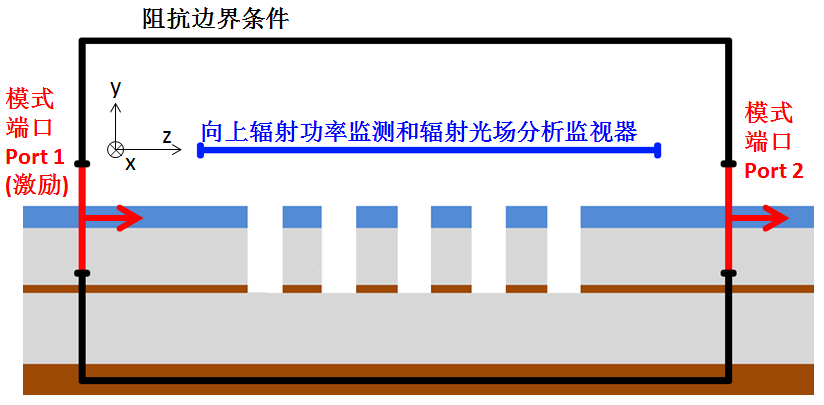
\includegraphics[width=1\textwidth]{Img/3-8.png}
    \caption{有限元仿真的建模示意图。左端的红色端口设置为电磁波的模式激励端口Port1,右端的红色端口设置为模式端口Port2,黑色的边界设置为阻抗边界条件,并离仿真区域10微米以上。在光栅的上方设置一个蓝色的Cutline,用于积分求解向上辐射的功率和提取向上辐射的电场的分布。}
    \label{fig:3-8}
\end{figure}
%%%%%%%%%%%%%%%%%%%%%%%%%%%%%%%%%%%%%%%%%%%%%%%%%%%%%%%%%%%%%%%%%%%%%%%%%%%%%%%%%%%%%%%%%%%%%%%%%%%%%%%%%%%%%%%%%%%%%%

如图3.8所示,在有限元的模型建立和仿真编程中,需要设置好光栅耦合器的仿真物理场、器件模型几何结构、材料属性、边界条件、求解器设置和仿真结果的预处理等模型配置。
 
大致的模型配置如下:

选择的物理场为波动光学Wave Optics或电磁波Electromagnetic Waves,求解器选择频域求解器Frequency Domain。

器件的大致模型几何结构如图3.8所示,其中淡蓝色的部分是氮化硅材料,设置的材料折射率为1.9894,而淡灰色的部分是氧化硅材料,设置的材料折射率为1.4431,棕红色的部分是硅材料,设置的材料折射率为3.42,纯白色部分为空气,设置的折射率为1。

仿真区域整体的黑色边界条件为阻抗边界条件,可以尽量不产生边界反射,并且距离仿真区域较远。在红色的边界处设置为端口Port,其中左端的端口Port1设置为激励端口,而波导右边输出端Port2设置为非激励端口,蓝色的切线Cutline距离光栅上表面2微米,用于积分求解向上辐射功率和提取向上辐射光场分析,用于耦合效率的中进行计算。在Port1激励端口输入对应的电磁波TE模式,TE模式的电场偏振态平行于x轴。

频域求解器设置好光波长或电磁波的频率,便可对光栅耦合器的稳态辐射电磁场分布进行求解。

通过如上方法设置好器件模型后,就可通过遗传算法对模型进行调用、仿真和数据处理,其具体的程序框图3.9所示。

在的全局变量中,设置好对应的变量,如光栅齿的宽度,光栅槽的宽度,氧化硅层厚度等,再通过遗传算法的优化程序,优化并求解光栅耦合器的结构变量。

\begin{figure}[!htbp]
    \centering
    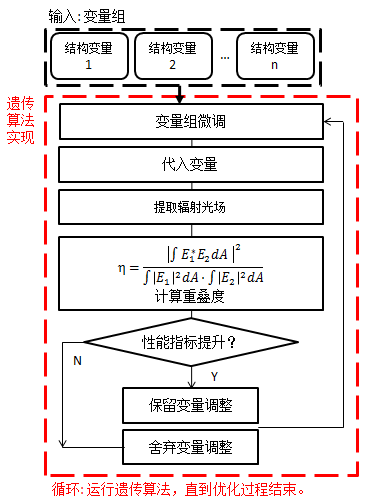
\includegraphics[width=0.8\textwidth]{Img/3-9.png}
    \caption{光栅耦合器模型进行遗传算法优化的大致程序流程。将待优化的结构变量,代入中进行仿真运算,再通过提取辐射光场和模式重叠度计算,计算光栅的耦合效率。并通过遗传算法进行循环迭代优化,实现效率的提升。}
    \label{fig:3-9}
\end{figure}
%%%%%%%%%%%%%%%%%%%%%%%%%%%%%%%%%%%%%%%%%%%%%%%%%%%%%%%%%%%%%%%%%%%%%%%%%%%%%%%%%%%%%%%%%%%%%%%%%%%%%%%%%%%%%%%%%%%%%%

如图3.9中,光栅耦合器仿真中,光栅耦合器的效率,通过如下公式计算

\begin{equation}
\eta= P_{up}\times \varepsilon
\end{equation}
其中$P_up$为向上辐射光的光功率,可通过电磁场能流线积分进行计算。沿着蓝色切线Cutline,积分能流的y分量,可以计算得到$P_{up}$。而$\varepsilon$为向上辐射的光场与标准单模光纤的光场的模式匹配度。模式匹配度$\varepsilon$可以通过提取切线Cutline的电场分布,并与单模光纤的准高斯模式进行模式匹配度计算,计算的公式如下:

\begin{equation}
\varepsilon= \frac{|\int{E_{up}^* E_{SMF}dz}|^2}{|\int{E_{up}dz}|^2| \int{E_{SMF}dz}|^2} 
\end{equation}

其中$E_{up}$为提取的向上辐射光的电场分布,$E_{SMF}$为的单模光纤的倾斜高斯模式,其公式为

\begin{equation}
E_{SMF}=A exp \left(-\frac{(z-z_0)^2}{w_0^2}\right)  exp \left(-in\frac{2\pi}{\lambda} sin \theta z \right)
\end{equation}

其中A为光纤模式的高斯模式的归一化常数,$w_0$为高斯模式的光腰半径,对于标准单模光纤,光腰半径为5.2$\mu$m,光纤的折射率n为1.46,而光纤的倾斜角度
θ = - 8 °。
通过上述仿真,设计和优化了两种常用的一步刻蚀的光栅耦合器,一种是加工容差特性较好的均匀光栅,一种是峰值效率更高的非均匀光栅。

\subsection{仿真结果}

\begin{figure}[!htbp]
    \centering
    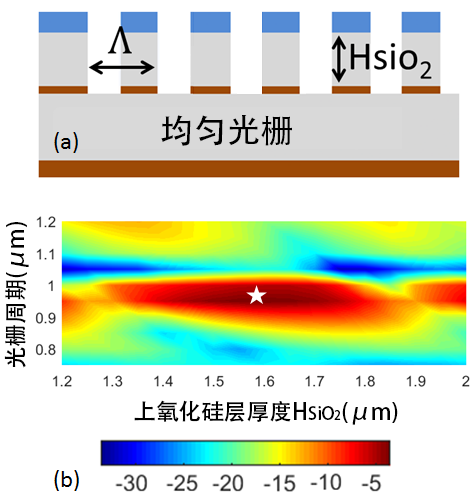
\includegraphics[width=0.8\textwidth]{Img/3-10.png}
    \caption{均匀光栅的仿真结果。(a) 均匀光栅的结构,在光栅优化过程中,考虑两个最主要的结构参数,光栅周期Λ和上氧化硅层的厚度Hsio2。(b)通过穷举仿真得到当光栅周期为0.95$\mu$m和上氧化硅层的厚度为1.6$\mu$m时,光栅耦合器的效率最高,为-3.52dB。}
    \label{fig:3-10}
\end{figure}
%%%%%%%%%%%%%%%%%%%%%%%%%%%%%%%%%%%%%%%%%%%%%%%%%%%%%%%%%%%%%%%%%%%%%%%%%%%%%%%%%%%%%%%%%%%%%%%%%%%%%%%%%%%%%%%%%%%%%%

通过上一小节的方法,主要设计和优化了两种的光栅耦合器,一种是加工容忍度高,带宽较宽,器件更稳定的均匀光栅的光栅耦合器,另一种是匹配单模光纤模式的具有更高峰值耦合效率的非均匀光栅的光栅耦合器。

如图3.10所示,考虑了均匀光栅的仿真,一般而言,均匀光栅的光栅耦合器相比非均匀光栅,光耦合的效率较低,然而具有更好的加工误差容忍度和更宽的光谱带宽,在实际的集成光子芯片中应用较为广泛。

本方案的均匀光栅,相关的结构变量较少,如图3.10,有氮化硅层的厚度Hsin、二氧化硅层的厚度Hsio2、光栅周期$\Lambda$,光栅占空比FF,光纤耦合角度θ等变量。

在芯片测试中,为便于测试,光纤耦合角度θ通常为5-20°的范围。本实验中,耦合角度选择-8°。为了提高光栅的最小特征尺寸,光栅占空比选定为50\%,便于光栅的曝光和刻蚀。氮化硅波导的厚度定为600nm,是出于反常波导色散设计。因此需要优化的器件结构变量有二氧化硅层的厚度Hsio2、光栅周期Λ,如图3.10a。

因此,采用了穷举优化的方法,即完全变量组合(All combination)的方法,优化了器件的二氧化层厚度Hsio2和光栅周期$\Lambda$,通过在MATLAB中改变光栅的周期和上层氧化硅层的厚度,并计算在C波段的中心波长1550nm波长时,光栅耦合器耦合效率随Hsio2和$\Lambda$变化的映射图,如图3.10b。从图中可以得到,当光栅的周期为0.95$\mu$m时,且上层氮化硅的厚度为1.6$\mu$m时,可以实现最高的均匀光栅效率为-3.52dB。

在此基础之上,进一步优化均匀光栅,可得,当光栅周期$\Lambda$=965nm时, FF=51.3\%时,均匀光栅的光栅耦合器具有最高的耦合效率,如图3.12所示。

\begin{figure}[!htbp]
    \centering
    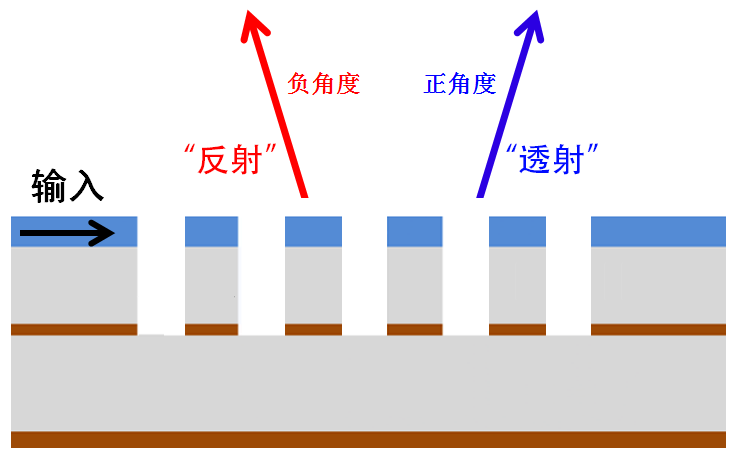
\includegraphics[width=0.8\textwidth]{Img/3-11.png}
    \caption{在光栅耦合器仿真时,之所以选择-8°的负数耦合角度,是因为在一步刻蚀的三层光栅结构中,光从波导输入近似于遭遇了垂直于芯片表面的DBR结构,因此形成“反射”比形成“透射”要更强烈。仿真结果也证明了负数角度的耦合效率更高。}
    \label{fig:3-11}
\end{figure}
%%%%%%%%%%%%%%%%%%%%%%%%%%%%%%%%%%%%%%%%%%%%%%%%%%%%%%%%%%%%%%%%%%%%%%%%%%%%%%%%%%%%%%%%%%%%%%%%%%%%%%%%%%%%%%%%%%%%%%

均匀光栅的耦合仿真中,光纤的耦合角度定为-8°,为反向的耦合角度。在仿真过程中也尝试过正向的耦合角度,然而仿真的结果不太好,耦合效率较低。本方案中的一步刻蚀的三层光栅结构,如图3.11所示,由于采用了深刻蚀的设计,刻蚀深度接近2.4$\mu$m,可以视作垂直于芯片表面的DBR结构。在DBR结构中,形成“反射”会比形成“透射”更具有优势,即负数的耦合角度比正的耦合角度更具优势。通过数值仿真的尝试,也能证实当耦合角度为负值时,耦合效率更高。因此,本实验中,选择了光栅耦合器的耦合角度为-8°。

\begin{figure}[!htbp]
    \centering
    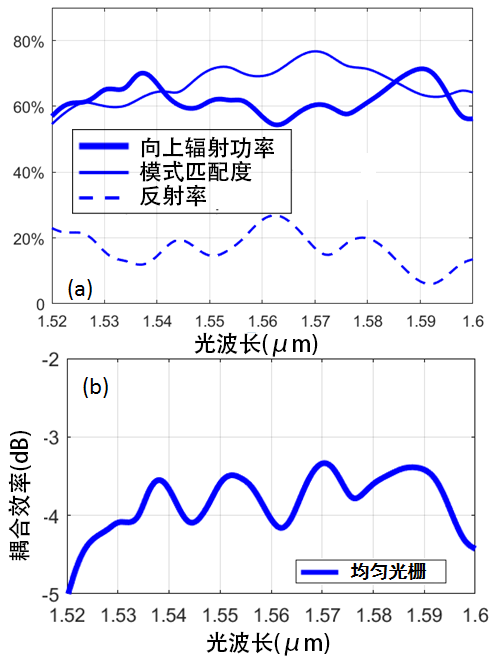
\includegraphics[width=0.8\textwidth]{Img/3-12.png}
    \caption{非均匀光栅的仿真结果。$\Lambda$=965nm,FF=51.3\%,Hsio2=1.6$\mu$m。(a) 波长扫描得到的光栅向上辐射效率、光栅辐射光场与单模光纤模式的匹配度和光栅波导的反射率。(b) 波长扫描得到的光栅耦合器偶和效率,可见峰值的耦合效率为-3.4dB,波长为1570nm,且1dB带宽超70nm。}
    \label{fig:3-12}
\end{figure}
%%%%%%%%%%%%%%%%%%%%%%%%%%%%%%%%%%%%%%%%%%%%%%%%%%%%%%%%%%%%%%%%%%%%%%%%%%%%%%%%%%%%%%%%%%%%%%%%%%%%%%%%%%%%%%%%%%%%%%

通过MATLAB脚本对光栅耦合器的波长响应进行仿真,如图3.12所示,在C波段附近1520-1600nm波长范围内,仿真了器件的光栅向上辐射效率、光栅辐射光场与单模光纤模式的匹配度和光栅波导的反射率。

通过向上辐射功率百分比和模式匹配度的乘积,可以计算得到从波导中耦合到单模光纤的效率。一般情况下,还要考虑光从空气耦合到单模光纤中的界面反射,然而由于单模光纤的折射率较低,空气—单模光纤界面的反射约为

\begin{equation}
\left( \frac{n_{SMF}-n_{air}}{n_{SMF}+n_{air}} \right)^2 \approx 4\%
\end{equation}

反射的比例较小可以忽略不计。可见,在C波段附近,1525-1595nm范围内耦合效率可以在-4.5dB以上,其1dB带宽为70nm,1dB带宽可以覆盖1525-1575nm的通信C波段范围,还覆盖部分L波段1575-1625nm的波长范围。在实际应用中,覆盖更宽的频谱范围,在通信、传感、声光非线性等应用中具有较大的意义。
 
均匀的光栅仍存在一些问题,如图3.12a,其仿真的器件反射率约为20\%,反射较大,反射驻波在通信应用中需要引入非线性光隔离器来避免反射的影响。因此,需要进一步优化均匀光栅,降低光栅反射。另一方面,也有利于进一步提高光栅耦合器的耦合效率。

\begin{figure}[!htbp]
    \centering
    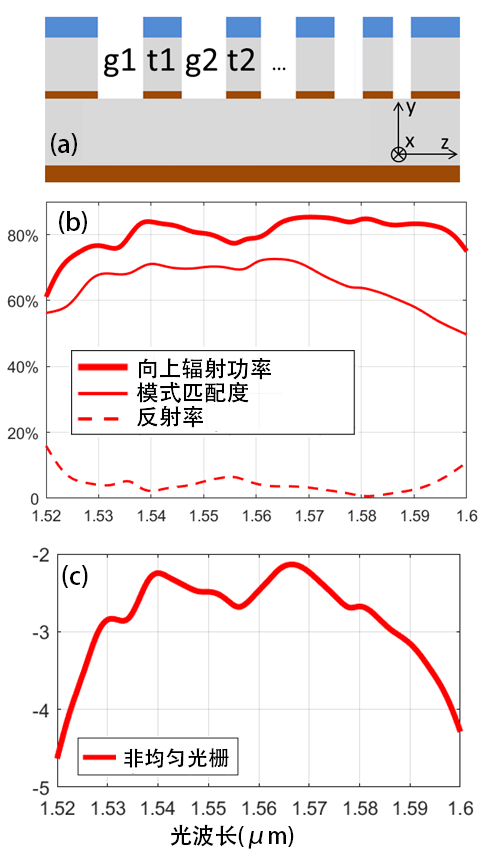
\includegraphics[width=0.8\textwidth]{Img/3-13.png}
    \caption{ 非均匀光栅的仿真结果,器件的结构变量见表3-2。(a) 非均匀非均匀光栅的变量定义。(b) 波长扫描得到的光栅向上辐射效率、光栅辐射光场与单模光纤模式的匹配度和光栅波导的反射率。(c) 波长扫描得到的光栅耦合器偶和效率,可见峰值的耦合效率为-2.1dB,波长为1568nm,且1dB带宽超65nm。}
    \label{fig:3-13}
\end{figure}
%%%%%%%%%%%%%%%%%%%%%%%%%%%%%%%%%%%%%%%%%%%%%%%%%%%%%%%%%%%%%%%%%%%%%%%%%%%%%%%%%%%%%%%%%%%%%%%%%%%%%%%%%%%%%%%%%%%%%%

如图3.13所示,均匀光栅的光栅耦合器的存在较高的波导反射率、较低耦合效率的局限,可以通过进一步的非均匀的非均匀光栅来优化。

在非均匀光栅中,由于每个光栅的齿和槽的宽度都可以视作是独立的变量进行优化,如图3.13a和表3-2,一个非均匀的光栅耦合器的变量有24个。当变量较多时,不能采用传统的穷举优化的变量优化方法,需要采用高效的多变量优化的算法,采用遗传算法来进行优化光栅的结构。具体的算法过程如图3.9所示。

通过遗传算法的优化,得到了表3-4中的光栅耦合器的几何结构变量


\begin{table}[!htbp]
    \caption{遗传算法优化得到的光栅耦合器几何结构变量(单位nm)}
    \label{tab:2}
    \centering
    \footnotesize% fontsize
    \setlength{\tabcolsep}{4pt}% column separation
    \renewcommand{\arraystretch}{1.2}%row space 
\begin{tabular}{cccccccc}
g1  & t1  & g2  & t2  & g3  & t3  & g4  & t4    \\ \hline
405 & 530 & 450 & 490 & 470 & 505 & 460 & 520   \\
g5  & t5  & g6  & t6  & g7  & t7  & g8  & t8    \\ \hline
545 & 440 & 555 & 475 & 495 & 475 & 515 & 460   \\
g9  & t9  & g10 & t10 & g11 & t11 & g12 & Hsio2 \\ \hline
525 & 540 & 465 & 415 & 510 & 495 & 430 & 1625 
\end{tabular}
\end{table}
%%%%%%%%%%%%%%%%%%%%%%%%%%%%%%%%%%%%%%%%%%%%%%%%%%%%%%%%%%%%%%%%%%%%%%%%%%%%%%%%%%%%%%%%%%%%%%%%%%%%%%%%%%%%%%%%%%%%%%
%%%%%%%%%%%%%%%%%%%%%%%%%%%%%%%%%%%%%%%%%%%%%%%%%%%%%%%%%%%%%%%%%%%%%%%%%%%%%%%%%%%%%%%%%%%%%%%%%%%%%%%%%%%%%%%%%%%%%%
%%%%%%%%%%%%%%%%%%%%%%%%%%%%%%%%%%%%%%%%%%%%%%%%%%%%%%%%%%%%%%%%%%%%%%%%%%%%%%%%%%%%%%%%%%%%%%%%%%%%%%%%%%%%%%%%%%%%%%

在表3-4的几何结构参数下,如图3.13b所示波长扫描,其中向上辐射的功率百分比接近85\%,且向上辐射的光功率与单模光纤的高斯模式的匹配度将近70\%,另一方面,光栅耦合器的波导反射也得到很好的缓解,反射功率也降低到5\%或-13dB以下。波长扫描仿真得到的波导到光纤的耦合效率如图3.13c所示,其中理论的峰值耦合效率为在-2.1dB@1568nm,且器件的1dB带宽约为65nm,覆盖需要的C波段光谱范围。

在设计均匀光栅和非均匀光栅的氮化硅光栅耦合器后,还需要度器件的容差特性进行分析。容差分析在器件设计和加工过程中非常重要,可以预知器件的性能随着加工误差或测试误差带来的变化,并对器件的加工可行性和可操作性做一个有效的评估。此外,在器件测试过程中,结合容差分析的趋势,可以对测试结果的展开合理的分析,并形成有意义的加工结果反馈。在本方案中,容易引起性能变化的主要加工误差有:光栅齿的刻蚀占空比变化情况、摆放光纤的位置偏差、以及中间的氧化硅层厚度的变化等。

如图3.14所示,对应的均匀光栅和非均匀光栅的误差分析。重点分析了当光纤放置位置偏差±4$\mu$m的情况下、当光栅齿的尺寸偏差±50nm的时候、以及当中间氧化硅层的厚度变化±0.1$\mu$m的时候,器件仿真的峰值光栅耦合器的峰值耦合效率的变化情况。,
其中,中间氧化硅层的厚度,可以通过气相外延生长时的陪片监控来实现精准厚度生长。而光纤位置可以通过三维台来控制。而光栅齿的占空比需要控制在±20nm(5\%)左右,在合理的电子束曝光序列控制的情况下,在器件曝光和刻蚀的过程注意控制刻蚀,同时结合改变光纤的摆放位置,来补偿光栅刻蚀带来的器件性能下降。理论上该加工容差可以在实验上实现,在下一节对光栅耦合器进行制备。

\begin{figure}[!htbp]
    \centering
    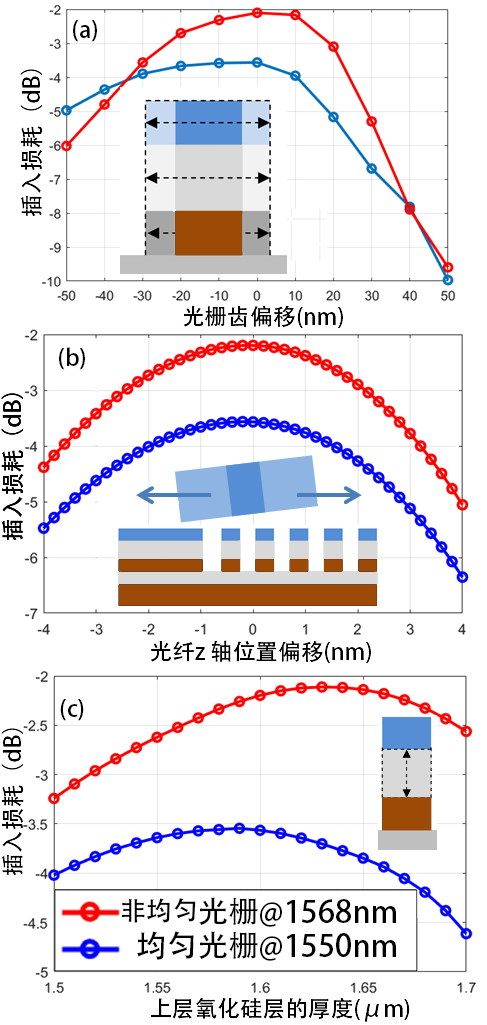
\includegraphics[width=0.7\textwidth]{Img/3-14.png}
    \caption{光栅耦合器的容差分析图。(a) 光栅齿的尺寸偏移对器件耦合效率的影响。(b)光纤摆放位置z轴偏移导致的耦合效率影响。(c)上氧化硅层厚度变化对器件耦合效率的影响。}
    \label{fig:3-14}
\end{figure}
%%%%%%%%%%%%%%%%%%%%%%%%%%%%%%%%%%%%%%%%%%%%%%%%%%%%%%%%%%%%%%%%%%%%%%%%%%%%%%%%%%%%%%%%%%%%%%%%%%%%%%%%%%%%%%%%%%%%%%


\subsection{器件加工与测试}

\begin{figure}[!htbp]
    \centering
    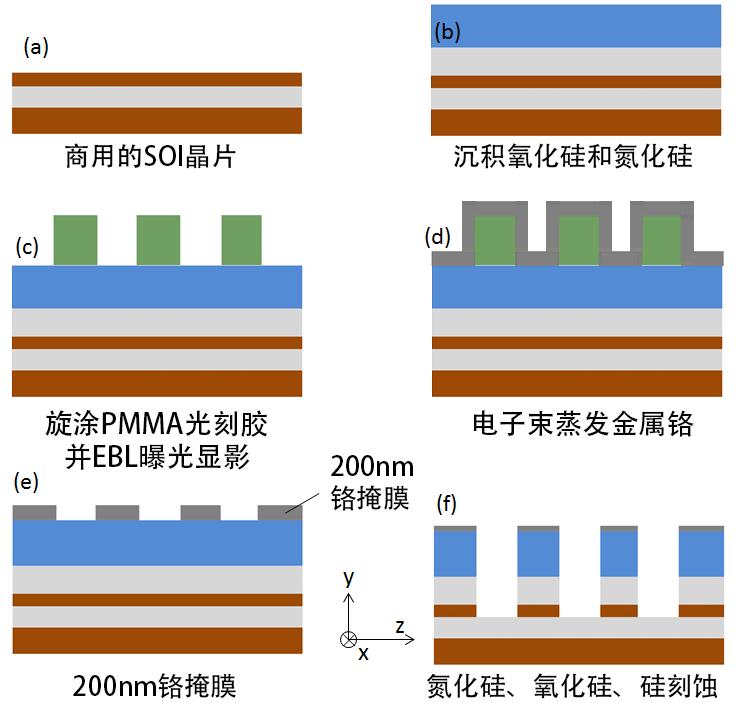
\includegraphics[width=1\textwidth]{Img/3-15.png}
    \caption{器件加工后的SEM和显微镜图。(a) 选用220nm硅层的SOI晶片。(b)在SOI晶片上沉积1600nm氧化硅和600nm氮化硅层。(c) 旋涂PMMA光刻胶并光刻显影得到PMMA掩膜。(d)通过电子束蒸镀,镀上200nm的金属铬。 (e) lift-off得到200nm厚的铬金属掩膜。(f)通过等离子体刻蚀,一步刻蚀氮化硅、氧化硅、硅层,完成光栅制备。}
    \label{fig:3-15}
\end{figure}
%%%%%%%%%%%%%%%%%%%%%%%%%%%%%%%%%%%%%%%%%%%%%%%%%%%%%%%%%%%%%%%%%%%%%%%%%%%%%%%%%%%%%%%%%%%%%%%%%%%%%%%%%%%%%%%%%%%%%%

器件的加工过程较为简单,如图3.15所示,只需要进行一次的光栅刻蚀过程就可以制备。器件加工流程中最大的挑战是实现2.5$\mu$m的光栅齿的刻蚀。传统的聚合物光刻胶难以实现接近1:6宽高比光栅的刻蚀,因此在本方案中,采用200nm的铬金属掩膜,通过金属掩膜的的超过1:20的的刻蚀选择比来实现深光栅的制备。

采用铬金属掩膜,是因为铬金属可以溶解于硝酸和硝酸四氨的混合溶液中,形成可溶的四氨合铬[Cr(NH3)4]3+络合物并去除,使用方法上类似于聚合物的去胶液。\cite{chromium}

而沉积200nm的金属铬掩膜,一般情况下需要有足够高,一般3-4倍以上厚度的聚合物光刻胶来lift-off实现,否则,光刻胶结构太薄,金属太厚容易造成金属粘连成片导致lift-off失败。因此,本试验采用了1100nm的PMMA正胶,通过EBL曝光显影,后真空蒸镀铬后lift-off的方法,形成金属铬掩膜。


形成铬金属掩膜之后,需要通过三次等离子体刻蚀,刻蚀的参数如下

\begin{table}[!htbp]
    \caption{首先通过反应离子束刻RIE刻蚀氮化硅600nm,表格为等离子体刻蚀的菜单}
    \label{tab:3}
    \centering
    \footnotesize% fontsize
    \setlength{\tabcolsep}{4pt}% column separation
    \renewcommand{\arraystretch}{1.2}%row space 
\begin{tabular}{|c|c|c|c|c|c|}
\hline
CHF3 & O2 & RF  & temp & press & time   \\ \hline
50   & 5  & 200 & 20   & 50    & 3'30'' \\ \hline
\end{tabular}
\end{table}

\begin{table}[!htbp]
    \caption{其次通过是RIE刻蚀二氧化硅1600nm,表格为等离子体刻蚀的菜单}
    \label{tab:4}
    \centering
    \footnotesize% fontsize
    \setlength{\tabcolsep}{4pt}% column separation
    \renewcommand{\arraystretch}{1.2}%row space 
\begin{tabular}{|c|c|c|c|c|c|}
\hline
CHF3 & Ar & RF  & temp & press & time    \\ \hline
12   & 12 & 200 & 20   & 30    & 23'30'' \\ \hline
\end{tabular}
\end{table}

\begin{table}[!htbp]
    \caption{最后通过电感耦合增强等离子体ICP刻蚀硅220nm,表格为等离子体刻蚀的菜单}
    \label{tab:5}
    \centering
    \footnotesize% fontsize
    \setlength{\tabcolsep}{4pt}% column separation
    \renewcommand{\arraystretch}{1.2}%row space 
\begin{tabular}{|c|c|c|c|c|}
\hline
HBr & ICP & temp & press & time \\ \hline
20  & 500 & 50   & 4     & 90'' \\ \hline
\end{tabular}
\end{table}
%%%%%%%%%%%%%%%%%%%%%%%%%%%%%%%%%%%%%%%%%%%%%%%%%%%%%%%%%%%%%%%%%%%%%%%%%%%%%%%%%%%%%%%%%%%%%%%%%%%%%%%%%%%%%%%%%%%%%%
%%%%%%%%%%%%%%%%%%%%%%%%%%%%%%%%%%%%%%%%%%%%%%%%%%%%%%%%%%%%%%%%%%%%%%%%%%%%%%%%%%%%%%%%%%%%%%%%%%%%%%%%%%%%%%%%%%%%%%
%%%%%%%%%%%%%%%%%%%%%%%%%%%%%%%%%%%%%%%%%%%%%%%%%%%%%%%%%%%%%%%%%%%%%%%%%%%%%%%%%%%%%%%%%%%%%%%%%%%%%%%%%%%%%%%%%%%%%%
则可以实现如图3.16c所示的电子显微镜SEM下的1:6宽高比的氮化硅+氧化硅+硅的三层光栅。


如图3.16a所示,还需要在刻蚀好的光栅的基础上再刻蚀氮化硅的波导.本实验设计的氮化硅光栅耦合器不需要精确的电子束对准套刻,使用海德堡$\mu$pg501无掩膜光刻机,其标称的套刻精度≥0.5$\mu$m,过程相对简单,并不影响器件的性能。刻蚀氮化硅的波导后的光栅耦合器如图3.16a所示。

\begin{figure}[!htbp]
    \centering
    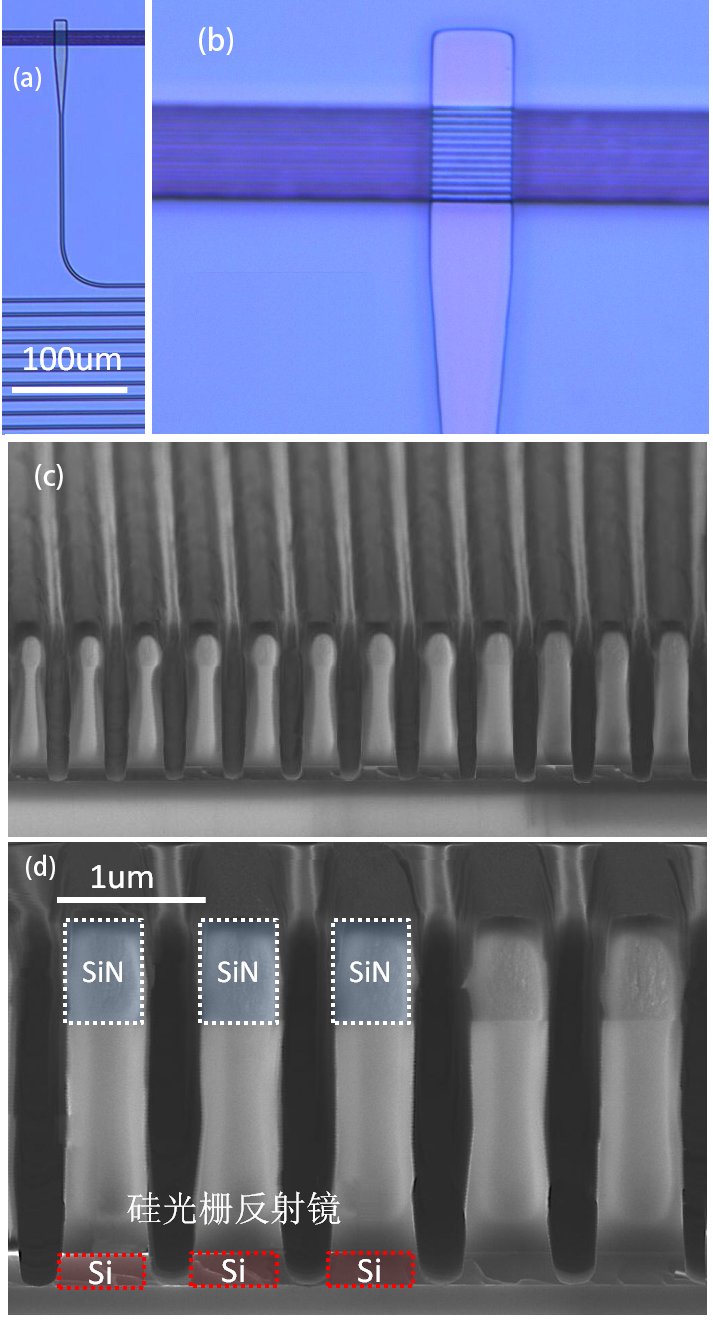
\includegraphics[width=0.8\textwidth]{Img/3-16.png}
    \caption{(a) (b) 制备后的光栅耦合器在光学显微镜下的图。(c)(d) 制备后的光栅耦合器在电子显微镜下的图,可以清晰的看到硅光栅反射镜和氮化硅的衍射光栅结构。}
    \label{fig:3-16}
\end{figure}
%%%%%%%%%%%%%%%%%%%%%%%%%%%%%%%%%%%%%%%%%%%%%%%%%%%%%%%%%%%%%%%%%%%%%%%%%%%%%%%%%%%%%%%%%%%%%%%%%%%%%%%%%%%%%%%%%%%%%%

图3.16为加工后的器件,对器件进行测试,本方案中光栅的耦合角度为-8度,在采用双边光栅耦合器的测试方案时,负数的耦合角度会有不便,因此,选择了一端为光栅耦合器,一端为锥形光纤端面耦合的方式,如图3.17c,其优点为,可以通过较短的光波导来实现测试,短的光波导意味着波导的传输损耗在后续的数据处理中忽略不计,简化了器件测试的过程。同时,器件面积小,可以在同个芯片上制备更多的样品,有利于测试。

\begin{figure}[!htbp]
    \centering
    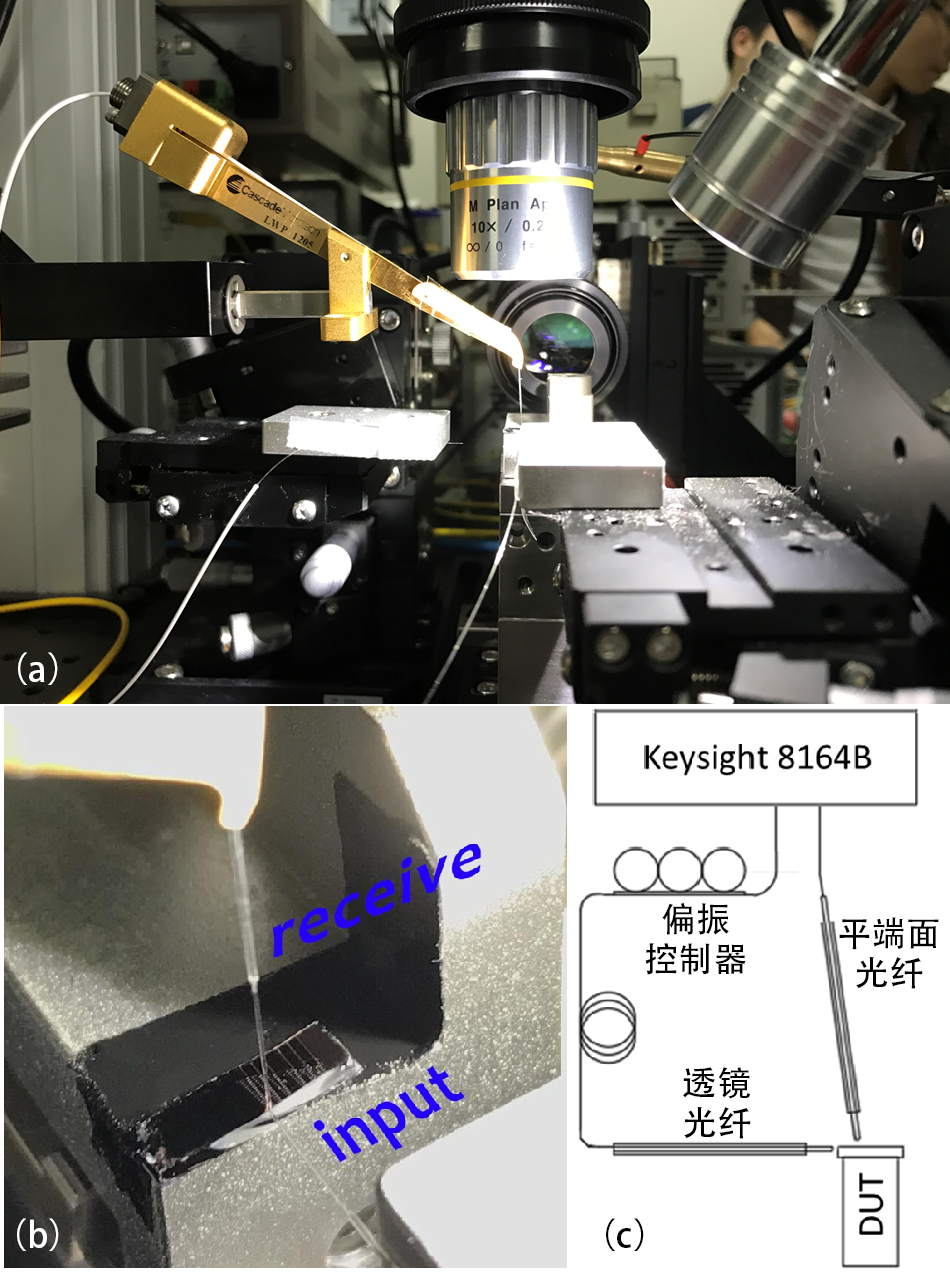
\includegraphics[width=0.8\textwidth]{Img/3-17.png}
    \caption{ (a) 光栅耦合器的大致测试装置。(b) 光从断面的锥形光纤输入,到光栅处衍射后,通过垂直的平端面单模光纤接收。(c) 测试链路的大致装置示意图。通过Keysight 8164B激光器进行波长扫描,完成器件测试。}
    \label{fig:3-17}
\end{figure}
%%%%%%%%%%%%%%%%%%%%%%%%%%%%%%%%%%%%%%%%%%%%%%%%%%%%%%%%%%%%%%%%%%%%%%%%%%%%%%%%%%%%%%%%%%%%%%%%%%%%%%%%%%%%%%%%%%%%%%

\begin{figure}[!htbp]
    \centering
    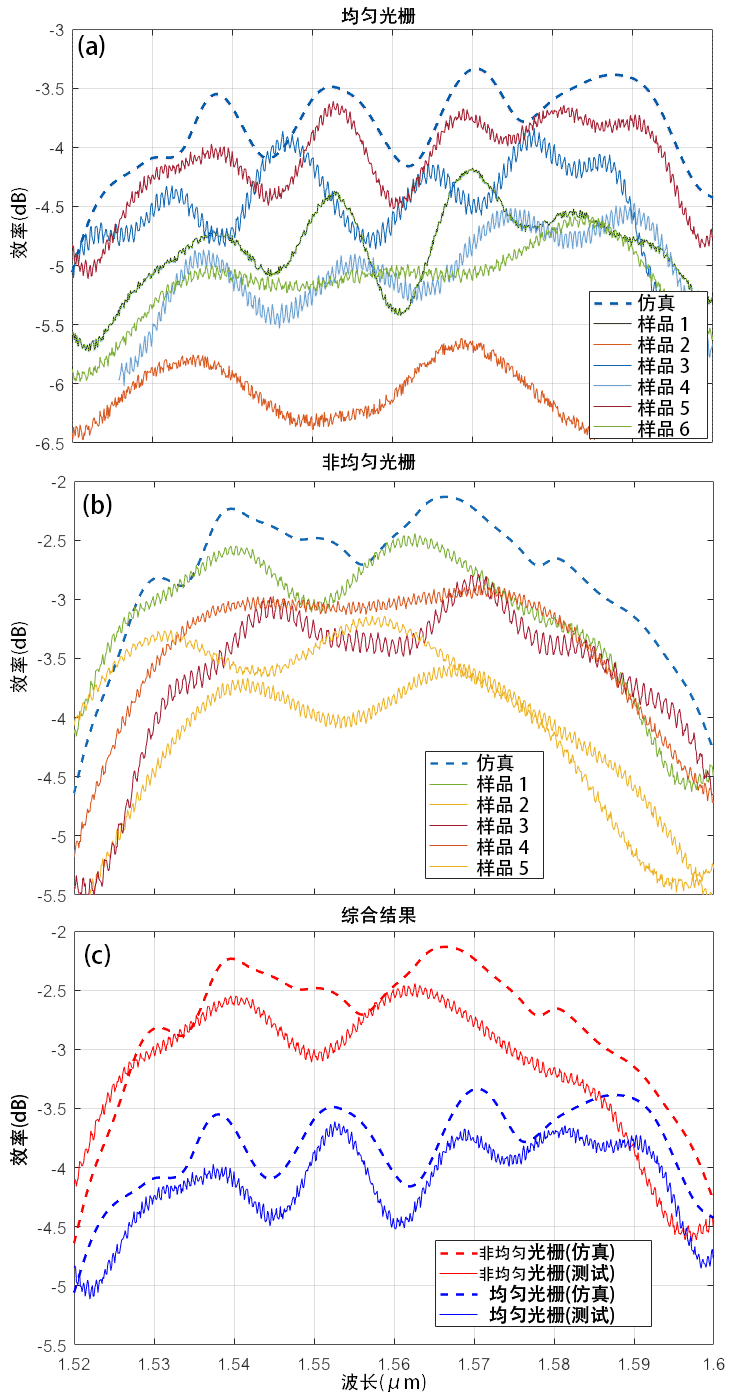
\includegraphics[width=0.8\textwidth]{Img/3-18.png}
    \caption{ 器件的测试结果图。(a)均匀光栅下测试样品的耦合效率和仿真的耦合效率。(b) 非均匀光栅下测试样品的耦合效率和仿真的耦合效率。(c) 最优的器件测试结果。}
    \label{fig:3-18}
\end{figure}
%%%%%%%%%%%%%%%%%%%%%%%%%%%%%%%%%%%%%%%%%%%%%%%%%%%%%%%%%%%%%%%%%%%%%%%%%%%%%%%%%%%%%%%%%%%%%%%%%%%%%%%%%%%%%%%%%%%%%%

器件测试的配置图如图3.17a所示,采用的是一端-8°垂直耦合,另一端为锥形光纤的端面耦合。示意图如3.17c所示。采用了8164B光波测量系统,产生了1550nm的激光,经过了光纤偏振控制器的偏振控制,耦合并激发波导中的TE模式,光波导中的光传输到衍射光栅后,向上辐射,通过上方的平端面的单模光纤进行接收,返回到8164B的光功率计上,完成功率监测,测试回路损耗。

图3.18是光栅耦合器的耦合损耗的测试结果。制备了不同曝光剂量的光栅耦合器样品,器件的测试的耦合损耗的抖动大致在1dB范围内,其中选取最佳的测试结果,其测试的结果与器件仿真的结果较为贴近。

\section{小结}
在本章中,提出并通过遗传算法设计了一种基于底部硅光栅反射镜的氮化硅光栅耦合器。通过下置式的硅光栅,实现较高的向上的辐射效率,从而极大的提升了器件的耦合效率。同时,又采用了一种便于制备的光栅一步刻蚀的方案,一方面保留了硅光栅反射镜的高效率,另一方面,避免了化学机械抛光CMP和高精度的电子束对准曝光HPA过程。并通过器件测试得到均匀光栅的耦合效率为-3.6dB和70nm的1dB带宽,而非均匀非均匀光栅的耦合效率为-2.5dB和65nm的1dB带宽。设计的氮化硅光栅耦合器,性能突出,制备简单,在实际的器件制备和应用中具有较高的应用前景。\cite{Xu2017High}
